\id{МРНТИ 52.47.25}{}

\begin{articleheader}
\sectionwithauthors{Ж.С. Саркулова, Г.А. Исенгалиева, Ж.Ж. Шильмагамбетова, Р.Ж. Оразбекова, А.М. Алиева}{ПОДБОР ОБОРУДОВАНИЯ ДЛЯ ЭКСПЛУТАЦИОННЫХ СКВАЖИН НА МЕСТОРОЖДЕНИИ КАРАГАНДА}

{\bfseries
Ж.С. Саркулова\textsuperscript{\envelope },
Г.А. Исенгалиева,
Ж.Ж. Шильмагамбетова,
Р.Ж. Оразбекова,
А.М. Алиева
}
\end{articleheader}

\begin{affiliation}
Актюбинский региональный университет им.К.Жубанова, Актобе, Казахстан

\raggedright \textsuperscript{\envelope } Корреспондент-автор: zhadi\_0691@mail.ru
\end{affiliation}

Подбор оборудования для эксплуатационных скважин на месторождении
Караганда включает в себя анализ геологических условий, выбор насосного
и трубопроводного оборудования, а также систем контроля и автоматизации.
Важно учитывать параметры нефти и газа, условия эксплуатации и
ремонтопригодность. Правильный выбор оборудования влияет на
эффективность добычи, снижение затрат и обеспечение надежности
процессов. Это требует детального анализа и часто подразумевает
сотрудничество с поставщиками для оптимизации решения.

Выбор оборудования и методов извлечения нефти осуществляется на основе
геолого-технических особенностей активных слоев, химических и физических
характеристик жидкости, а также условий эксплуатации, режимов работы
скважин, определяемых предполагаемым способом разработки.

Подбор наиболее оптимального метода механизированной эксплуатации
определяется различными факторами.Начало формы Важными из них являются
глубина залегания продуктивного горизонта, продуктивность скважины,
сложности, присущие эксплуатации конкретной скважины, а также
экономическая целесообразность оснащения скважины определенным
оборудованием.

Техническое и экономическое оправдание эксплуатации плунжерными
штанговыми насосами остается актуальным для средне и низкопродуктивных
скважин. В каждом конкретном случае подбор оборудования и оптимизация
режимов работы штанговой насосной установки осуществляется лично,
учитывая дебит, обводненность и газосодержание конкретной скважины на
месторождении. Эксплуатация плунжерными штанговыми насосами является
эффективным и рациональным способом разработки скважин, предоставляя
широкие возможности как для поверхностной добычи, так и для подъема
продукции с большой глубины.

{\bfseries Ключевые слова:} эксплуатационные скважины, оборудование для
бурения, автоматизированный метод, электроцентробежные насосы, винтовые
насосы, эффективность.

\begin{articleheader}
{\bfseries SELECTION OF EQUIPMENT FOR PRODUCTION WELLS AT THE KARAGANDA FIELD}

{\bfseries
Zh.S. Sarkulova\textsuperscript{\envelope },
G.A. Isengalieva,
Zh.Zh. Shilmagambetova,
R.ZH. Orazbekova,
A.M. Alieva
}
\end{articleheader}

\begin{affiliation}
Aktobe Regional University named after K.Zhubanov, Aktobe, Kazakhstan

e-mail: \href{mailto:zhadi\_0691@mail.ru}{zhadi\_0691@mail.ru}
\end{affiliation}

The selection of equipment for production wells at the Karaganda field
includes the analysis of geological conditions, the selection of pumping
and pipeline equipment, as well as control and automation systems. It is
important to take into account the parameters of oil and gas, operating
conditions and maintainability. The right choice of equipment affects
the efficiency of production, reducing costs and ensuring the
reliability of processes. This requires detailed analysis and often
involves collaboration with suppliers to optimize the solution.

The choice of equipment and methods of oil extraction is based on the
geological and technical characteristics of the active layers, chemical
and physical characteristics of the liquid, as well as operating
conditions, operating modes of wells determined by the proposed method
of development.

The selection of the most optimal method of mechanized operation is
determined by various factors. The most important of them are the depth
of the productive horizon, the productivity of the well, the
difficulties inherent in the operation of a particular well, as well as
the economic feasibility of equipping the well with certain equipment.

The technical and economic justification for the operation of plunger
rod pumps remains relevant for medium and low-productivity wells. In
each specific case, the selection of equipment and optimization of the
operating modes of the rod pumping unit is carried out personally,
taking into account the flow rate, water content and gas content of a
particular well in the field. The operation of plunger rod pumps is an
efficient and rational way to develop wells, providing ample
opportunities for both surface production and lifting products from
great depths.

{\bfseries Keywords:} production wells, drilling equipment, automated
method, electric centrifugal pumps, Screw pumps, efficiency.

\begin{articleheader}
{\bfseries ҚАРАҒАНДЫ КЕН ОРНЫНДА ПАЙДАЛАНУ ҰҢҒЫМАЛАРЫНА АРНАЛҒАН
ЖАБДЫҚТАРДЫ ІРІКТЕУ}

{\bfseries
Ж.С. Саркулова\textsuperscript{\envelope },
Г.А. Исенгалиева,
Ж.Ж. Шильмагамбетова,
Р.Ж. Оразбекова,
А.М. Алиева
}
\end{articleheader}

\begin{affiliation}
Қ.Жұбанов атындағы Ақтөбе өңірлік университеті, Ақтөбе қ., Қазақстан.

e-mail: \href{mailto:zhadi\_0691@mail.ru}{\nolinkurl{zhadi\_0691@mail.ru}}
\end{affiliation}

Қарағанды кен орнындағы пайдалану ұңғымалары үшін жабдықтарды іріктеу
геологиялық жағдайларды талдауды, сорғы және құбыржол жабдықтарын,
сондай-ақ басқару және автоматтандыру жүйелерін таңдауды қамтиды. Мұнай
мен газдың параметрлерін, пайдалану жағдайлары мен қызмет ету мерзімін
ескеру маңызды. Жабдықты дұрыс таңдау өндіріс тиімділігіне әсер етеді,
шығындарды азайтады және процестердің сенімділігін қамтамасыз етеді. Бұл
егжей-тегжейлі талдауды қажет етеді және көбінесе шешімді оңтайландыру
үшін жеткізушілермен ынтымақтастықты қамтиды.

Мұнай өндірудің жабдықтары мен тәсілдерін таңдау белсенді қабаттардың
геологиялық-техникалық сипаттамаларына, сұйықтықтың химиялық және
физикалық сипаттамаларына, сондай-ақ пайдалану жағдайларына,
ұңғымалардың жұмыс режимдеріне негізделген.

Механикаландырылған пайдаланудың ең оңтайлы әдісін таңдау әртүрлі
факторлармен анықталады. Олардың маңыздылары - өнімді горизонттың
тереңдігі, ұңғыманың өнімділігі, белгілі бір ұңғыманы пайдалануға тән
қиындықтар, сондай-ақ ұңғыманы белгілі бір жабдықтармен жабдықтаудың
экономикалық орындылығы.

Поршеньді штангалық сорғыларды пайдаланудың техникалық және экономикалық
негіздемесі орташа және төмен өнімді ұңғымалар үшін өзекті болып қала
береді. Әрбір нақты жағдайда штангалық сорғы қондырғысының жабдықтарын
таңдау және жұмыс режимдерін оңтайландыру кен орнындағы нақты ұңғыманың
дебитін, сулануын және газ құрамын ескере отырып, жеке жүзеге асырылады.
Поршеньді штангалық сорғыларды пайдалану Ұңғымаларды өңдеудің тиімді
және ұтымды әдісі болып табылады, бұл жер үсті өндіруге де, өнімді үлкен
тереңдіктен көтеруге де кең мүмкіндіктер береді.

{\bfseries Түйін сөздер:} пайдалану ұңғымалары, бұрғылау жабдықтары,
автоматтандырылған әдіс, электр ортадан тепкіш сораптар, бұрандалы
сораптар, тиімділік.

\begin{multicols}{2}
{\bfseries Введение.} Карагандинское месторождение расположено в
Каркаралинском районе Карагандинской области Казахстана. Рельеф
региона характеризуется мелкосопочным и низкогорным рельефом с
относительными превышениями до 50 метров.  Физико-химические свойства
нефти Карагандинского месторождения включают высокое содержание
парафиновых углеводородов. Содержание парафиновых углеводородов
нормального строения в два раза ниже по сравнению с изопарафинами, а
ароматических углеводородов в два раза больше, чем в нефти
Кенкиякского месторождения. Нефть этого месторождения является
малосернистой, с содержанием серы около 0,24\%. Удельный вес нефти
составляет 0,8256 г/см³. Выход фракций, выкипающих до 200 °C,
составляет 22\%, а до 300 °C — 48\%. Содержание сернокислотных смол
достигает 9\%.

Изучение информации о работе скважин позволило выявить ключевые факторы,
характерные для данного месторождения, которые оказывают влияние на
выбор оптимального метода эксплуатации:

- продуктивные горизонты в среднем залегают на глубине до 750 метров;

- давление в пластах юрских горизонтов варьируется от 1,54 до 5,82 МПа,
а в триасовых горизонтах от 2,45 до 4,67 МПа;

- давление, при котором нефть насыщается газом, находится в диапазоне от
0,2 до 1,54 МПа;

- газовое содержание в нефти юрских горизонтов низкое, составляющее от
1,5 до 5,22 м\textsuperscript{3}/т, в то время как для триасовых
горизонтов оно немного выше, в диапазоне от 4,68 до 10,88
м\textsuperscript{3}/т;

- нефть, добываемая с юрских горизонтов, характеризуется как тяжелая и
высоковязкая, с вязкостью от 80,7 до 505 мПа*с в зависимости от
конкретного пласта (от Горизонта Ю-II А до Горизонта Ю-IА). Кроме
того, она содержит парафин (до 4,45\% по массе) и смолу (до 16,6\% по
массе);

- при эксплуатации скважин наблюдается высокая интенсивность
пескопроявления, при этом содержание механических примесей в
добываемой продукции составляет от 0,001 до 0,25
г/м\textsuperscript{3};

- Продуктивность скважин характеризуется как средняя и низкая.
Пониженное содержание газа и высокая вязкость нефти, включая объекта
Ю-IA, оказывают влияние на реологические свойства нефти, которые
определяются большим количеством смол и асфальтенов. Это создает
определенные ограничения при выборе метода добычи. Фонтанный метод
добычи является наиболее экономически эффективным и менее сложным
методом добычи нефти из скважин с применением природной энергии пласта.
Однако, чтобы достичь проектного дебита при использовании фонтанного
метода, необходимы определенные факторы, такие как высокое пластовое
давление, наличие газа и коэффициент продуктивности скважин {[}1-2{]}.
Когда эти факторы отсутствуют или не удовлетворяются, не будет
достигнуто запланированное дебитирование нефти фонтанным методом. В
таких случаях, когда условия пласта не позволяют поддерживать приемлемый
уровень добычи или вообще препятствуют притоку пластовых флюидов в
скважину, требуется перевод скважин на механизированную добычу.

{\bfseries Материалы и методы.} В результате интерпретации результатов
комплексного пластового исследования было выявлено, что продуктивность
скважин на месторождении варьирует в диапазоне от 0,039
м\textsuperscript{3}/сут*атм. (скв.10) до 1,78
м\textsuperscript{3}/сут*атм. (скв.34). Забойное давление при испытании
скважин на Ю-IA горизонтах колеблется от 0,58 до 2,6 МПа, на горизонтах
Ю-II от 3 до 3,8 МПа, а на триасовых горизонтах составляет 3,6-4,9 МПа.
Анализ данных показал, что скважины, пробуренные на горизонте Ю-I, имеют
наибольшую депрессию на пласт, следовательно, проявляют более низкие
показатели продуктивности. Важно отметить, что физико-химические
свойства нефти на Ю-I горизонте существенно отличаются (низкое
содержание газа, высокая вязкость), что условия эксплуатации данного
объекта требуют режима с повышенной депрессией.

С целью установлений условий начального прорыва скважин, когда забойное
давление ожидается давление ниже точки насыщения нефти газом, были
проведены гидравлические расчеты с использованием аналитического
подхода, разработанного академиком Крыловым. Для фонтанирования скважин
при условии Р\textsubscript{заб}  Р\textsubscript{нас},
требуется, чтобы эффективный газовый фактор Г\textsubscript{эф} был не
менее удельного расхода газа на оптимальном режиме R\textsubscript{опт},
т. е.:

Г\textsubscript{эф}  R\textsubscript{опт} (1)

Коэффициент газонасыщенности Г\textsubscript{эф} и требуемый
индивидуальный расход газа R\textsubscript{опт} составляют 3,6
м\textsuperscript{3}/сут и 2704 м\textsuperscript{3}/сут вследствие
этого, при низком давлении на устье скважины 0,1 МПа и при давлении на
забое, близком к давлению насыщения. Это свидетельствует о недостаточных
условиях для естественного притока в скважину, так как связь между
коэффициентом газонасыщенности и индивидуальным расходом газа для
подъема жидкости состоит в том, что чем больше коэффициент
газонасыщенности, тем больше газа потребуется для эффективной добычи
жидкости из скважины {[}3{]}.

Согласно рекомендованному четвертому варианту разработки данной
технологической схемы, предусматривается проведение дополнительного
разбуривания 39 скважины, предназначенные для добычи, а также активация
5 скважин. Также планируется провести восстановительные работы и вывести
из утилизационного фонда 1 скважину с последующим переводом 23 скважин
на нагнетание. В целом, существующий фонд эксплуатационных скважин,
запланировано увеличить до 50 единиц в 2015 году, а затем снизить его до
30 скважин (2034) г.
\end{multicols}



\(N = \frac{Q \bullet \rho \bullet g \bullet H}{\eta \bullet 10^{6}}\)

\[N = \frac{50 \bullet 825,6 \bullet 9,81 \bullet 750}{0,5 \bullet 10^{6}} \approx 606,5\ кВт\]

\(\frac{Q}{Q_{\max}} = 1 - 0,2 \bullet \left( \frac{P_{wf}}{P_{r}} \right) - 0,8\ \left( \frac{P_{wf}}{P_{r}} \right)^{2}\)

\[\frac{Q}{50} = 1 - 0,2 \bullet \left( \frac{1,8}{3,8} \right) - 0,8\ \left( \frac{1,8}{3,8} \right)^{2}\]

\begin{figure}[H]
	\centering
	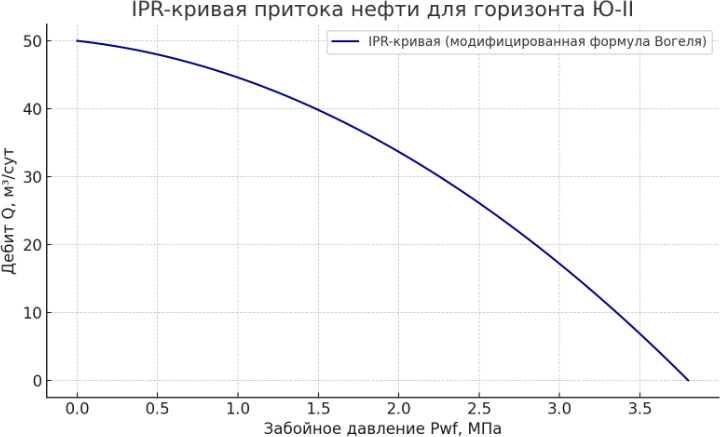
\includegraphics[width=0.8\textwidth]{media/gorn/image2}
	\caption*{}
\end{figure}

\begin{multicols}{2}
Автоматизированный метод насосной добычи нефти обычно реализуется через
три основных способа:

- установками плунжерных штанговых насосов (УПШН);

- установками электроцентробежных насосов (УЭЦН);

- установками винтовых штанговых насосов (УВШН).

Использование плунжерных штанговых насосов (УПШН) является эффективным
способом эксплуатации скважин, обеспечивая добычу в диапазоне от 2 до 80
м\textsuperscript{3}/сут и возможность подъема добычи из глубин свыше
2000 метров. Штанговые установка пользуются широким спросом благодаря
своей простоте конструкции, хорошо изученности и удобству использования,
что обеспечивает их рекомендацию для эксплуатации низко- и
среднедебитных скважин {[}4-5{]}.
\end{multicols}


%% \begin{longtable}[]{@{}
%%   >{\centering\arraybackslash}p{(\linewidth - 10\tabcolsep) * \real{0.2200}}
%%   >{\centering\arraybackslash}p{(\linewidth - 10\tabcolsep) * \real{0.2081}}
%%   >{\centering\arraybackslash}p{(\linewidth - 10\tabcolsep) * \real{0.0977}}
%%   >{\centering\arraybackslash}p{(\linewidth - 10\tabcolsep) * \real{0.1313}}
%%   >{\centering\arraybackslash}p{(\linewidth - 10\tabcolsep) * \real{0.1924}}
%%   >{\centering\arraybackslash}p{(\linewidth - 10\tabcolsep) * \real{0.1505}}@{}}
%% \toprule\noalign{}
%% \begin{minipage}[b]{\linewidth}\centering
%% {\bfseries Насос}
%% \end{minipage} & \begin{minipage}[b]{\linewidth}\centering
%% {\bfseries Производительность (м³/сут)}
%% \end{minipage} & \begin{minipage}[b]{\linewidth}\centering
%% {\bfseries Глубина (м)}
%% \end{minipage} & \begin{minipage}[b]{\linewidth}\centering
%% {\bfseries Тип нефти и условий работы}
%% \end{minipage} & \begin{minipage}[b]{\linewidth}\centering
%% {\bfseries Преимущества}
%% \end{minipage} & \begin{minipage}[b]{\linewidth}\centering
%% {\bfseries Ограничения}
%% \end{minipage} \\
%% \midrule\noalign{}
%% \endhead
%% \bottomrule\noalign{}
%% \endlastfoot
%% УПШН (Плунжерные штанговые насосы) & 2-80 & До 2000 & Низкая и средняя
%% дебитность & Простота, хорошая известность, удобство эксплуатации &
%% Меньше эффективны на больших глубинах \\
%% УЭЦН (Электроцентробежные насосы) & 60-1500 & 1000-3000 & Высокие
%% дебиты, высокая температура, вода и газ & Высокая производительность на
%% высокодебитных скважинах & Потери эффективности при высоких температурах
%% и газе \\
%% УВШН (Винтовые штанговые насосы) & 1-750 & Более 2000 & Трудоемкая,
%% вязкая нефть & Эффективны при вязкой нефти, перекачка твердых частиц &
%% Высокая стоимость установки и обслуживания \\
%% \end{longtable}

\begin{multicols}{2}
{\bfseries Результаты и обсуждение.} В процессе разработки предполагается
достижение максимального среднегодового дебита скважин по жидкости в
размере 75,8 т/сут к 2025 году. Стремительная эффективность эксплуатации
скважин при неполном насыщении пластовой нефти может предполагаться,
поскольку она позволяет создать достаточно высокую депрессию в пласте.

При наличии повышенного уровня газа в нефти и при эксплуатации с
уменьшенным Р\textsubscript{нас} забойными давлениями, постановка
насосов должна быть оснащена газозащитными устройствами.

Перевод скважин на работу с помощью плунжерных насосов предпочтительно
осуществлять с использованием вставных насосов следующих диаметров: 32,
38 и 44 мм. Также эффективными в этом процессе являются трубные насосы с
диаметрами 32, 38, 44 и 57 мм. Для этих насосов подходят
насосно-компрессорные трубы размером 73 мм. Стержень следует иметь
двухступенчатую конструкцию с диаметрами
7/8''{} и
3/4''. При откачке желательно выбирать
длинноходовый и низкочастотный режим, что обусловлено инертностью вязкой
нефти.

Способ использования установок электроцентробежных насосов (УЭЦН) для
эксплуатации скважин обеспечивает значительные преимущества по
сопоставлению с системами плунжерных штанговых насосов. Он наиболее
широко применяется на месторождениях, где вероятно произвести извлечение
от 60 до 1500 м\textsuperscript{3}/сут {[}6-7{]}.

На сегодняшний день производители установок электроцентробежных насосов
выпускают их с целью разнообразия условий эксплуатации. Рекомендуется
учитывать, что производительность внедрения таких установок также
понижена из-за возможного влияния высших температур
(\textgreater90\textsuperscript{0}С) на работу оборудования или высокого
содержания газа в добычи. Во многих ситуациях установки
электроцентробежных насосов эффективны в погружных скважинах с высоким
содержанием воды и дебитами жидкостей больше 50
м\textsuperscript{3}/сут. Однако, в процессе добыче плотной нефти,
использование установок электроцентробежных насосов может сопровождаться
значительным падением коэффициента эффективного воздействия насоса. При
пробном этапе применение установок электроцентробежных насосов не
является целесообразным для достижения прогнозных уровней добычи,
поскольку ожидаемые дебиты можно получить с помощью установок плунжерных
и винтовых насосов с уменьшенными капитальными и эксплуатационными
издержками.

Винтовые насосы стали очень популярными благодаря их способности
перекачивать флюиды, содержащие большое количество твёрдых частиц. Они
также отличаются своими свойствами, которые в некоторых аспектах схожи с
ароматическими соединениями газового конденсата. Винтовые насосы
способны эффективно перекачивать тяжелые эмульсии и нефть. Эти насосные
агрегаты имеют производительность от 1 до 750 м\textsuperscript{3}/сут и
могут работать в значительном содержании воды, не боясь песка и
абразивов.

В виду с потребностью разработки технических средств для добычи
трудоемкой и вязкой нефти, рекомендуется использовать
высокодепрессионный режим на месторождении Ю-1А, что позволяет снизить
забойное давление ниже давления насыщения. Одним из наиболее эффективных
методов, рассматриваемых для применения, называется способ холодильных
добычи тяжелой нефти с одновременным переносом песка. Опыт применения
данной технологии на аналогичных месторождениях показал, что
использование винтовых плунжерных насосов является наиболее эффективным
подходом. Этот тип установок наилучшим образом соответствует основным
принципам НТДТНП:

- в процессе извлечении нефти, вода и газ, а также песок и другие
твердые литологические материалы извлекаются совместно;

- в процессе добычи нефти в ствол скважины осуществляется поступление
песчаных частиц. Это происходит в результате создания высокого
давления на пласт, вызывающего значительное снижение забойного
давления до уровня ниже давления насыщения;

- в процессе эксплуатации установки винтовых штанговых насосов возникают
депрессии, которые влияют на формирование эмульсий. Тем не менее,
использование данной технологии позволяет снизить издержки на
переработку продукции.
Преимущества УВШН в сравнении с дополнительными машинными системами
называются следующими: низкие инвестиции, меньшие эксплуатационные
расходы относительно технического обслуживания установок, возможность
выбора эффективного материала из каучука, учитывая свойства извлекаемой
жидкости, а также отсутствие заслонок и, как следствие, сложности их
ударотермической неплотности. Благодаря своей апатичности к вольному
газу, винтовые насосы прекрасно соответствует для передачи
высокоуглеродистой нефти. Оборудование винтовых насосов преимущественно
стойкие к изнашиванию при приобритении масла с механическими примесями,
потому что твердые гранулы, передаваемые сквозь насос, давятся к
искривленной, но стойкой сетке эластомера (статора).

При выборе винтовых насосов по производительности необходимо учитывать
проектные уровни добычи нефти. В связи с этим, насосы отбираются с
большей производительностью, чем предполагаемый дебит, учитывая, что они
не смогут функционировать на предельных скоростях поворота. Для добычи
липкой нефти наилучшей скоростью вращения имеет 60-150 оборотов в
минуту. Рекомендуется устанавливать насос в нижней части интервала
перфорации. Чтобы обеспечить перемешивание поступающего потока,
предпочтительно применять хвостовик с прорезями длиной 0,5-1 м или
отверстиями диаметром 20 мм в основании насоса. Для обеспечения
безопасности ротора (в случае обрыва штанги) целесообразно монтировать
металлический брус снизу. Имеется зумпфа позволяет начать добычу при
больших дебитах песка, поскольку оно наполняется песком впоследствии
пуска скважины {[}8-9{]}.

В роли подъёмника используются НКТ диаметром 73 мм, которые опускаются в
эксплуатационную колонну диаметром 168 мм. Глубина опускания
насосно-компрессорных труб находится выше перфорированного интервала,
обычно на 10-20 метров. Если скважина оснащена насосными установками для
контроля активного и пассивного уровней, то кольцевое пространство
остается без изоляции пакером.

При выборе винтовых насосов для проектов добычи нефти, основываясь на
производительности, специалисты рекомендуют учитывать не только
ожидаемый дебит, но и уровни добычи. В этом случае рекомендуется
использовать насосы с большей производительностью, учитывая, что они не
будут функционировать на предельных скоростях вращения ротора (250-300
оборотов в минуту). В случае вязкой нефти, идеальной скоростью обращения
считается 60-150 оборотов в минуту, при этом она может меняться в
зависимости от крутящего момента в приводной системе. Обходя возможность
использования наземных приводов и штанг, можно опробовать винтовые
насосы с электрическими и гидравлическими погружными управляемые
системами, которые позволят регулировать крутящий момент и расход в
соответствии с уровнем жидкости в кольцевом полости. Кроме того, можно
использовать насосы с частотным контроллером скорости оборотов
электромотора, без необходимости переключение шкивов.

{\bfseries Выводы.} В процессе тестирования и эксплуатации на
Карагандинском месторождении был накоплен ценный опыт по работе
скважинных установок данного типа. В экспериментальных условиях были
использованы механизированные винтовые штанговые насосы, позволяющие
эффективно добывать нефть. На сегодняшний день компания "Протекс"
внедряет новые скважинные установки, которые обладают
производительностью от 10 до 17 м\textsuperscript{3}/сут при 100
оборотах в минуту и напором до 1200 метров. Статоры насосов имеют
эластомером типа РХ40, специально разработанным для работы в средах с
высокими температурами до 120 градусов, а также обладающим устойчивостью
к шлифовочными частицами, газам, запаховом веществом, серой и
углекислому газу {[}10-12{]}.

Оптимальное размещение винтового насоса предполагает его установку под
самыми нижними перфорациями отверстий на насосно-компрессорные трубы
диаметром 73-89 мм. Предлагается развивать такой промежуток
(\textasciitilde1м) между статором и перфорационными отверстиями в
соотношении с результативности конкретного винтового насоса. Это
обеспечивает оптимальную проходимую мощность и ограничивает крутящий
момент, обеспечивая эффективную работу насоса:

- для эффективного смешивания притока жидкости в основание насоса
советуются применять хвостовик с надрезами, длиной от 0,5 до 1м, или
же отверстиями диаметром 20 мм;

- для защиты ротора (в случае обрыва штанги) рекомендуется установить
стальной щит;

- наличие зумпфа с 1-4 трубами диаметром 168 мм в операционной колонне
обеспечивает быстрому запуском производства песка при больших
начальных дебитах;

- для более эффективной предотвращении раскручивания статора
рекомендуется устанавливать приспособление в верхнем участке;

- опускание ротора производится с использованием штанг диаметром 22 мм,
учитывая низкую глубину и крутящий момент;

- установка винтовых насосов с устройствами регулярного наблюдения за
вращающим поворотом.
\end{multicols}

\begin{center}
{\bfseries Литература}
\end{center}

\begin{references}
1. Котик Е.П., Котик П.Т. Разработка и эксплуатация нефтяных и газовых
месторождений: учебник. -Алматы:CyberSmith, 2021. --Т.1. -220 с. ISBN
978-601-342-948-9

1. Котик Е.П., Котик П.Т. Разработка и эксплуатация нефтяных и газовых
месторождений: учебник. -Алматы:CyberSmith, 2021. --Т.2. -212 с. ISBN
978-601-342-948-9

1. Котик Е.П., Котик П.Т. Разработка и эксплуатация нефтяных и газовых
месторождений: учебник. -Алматы:CyberSmith, 2021. --Т.3. -240 с. ISBN
978-601-342-948-9

1. KASE: нефтегазовая отрасль Республики Казахстан {[}Электронный
ресурс{]}. URL:
\href{https://kase.kz/files/presentations/ru/KASE_OilGas_industry_2019.pdf}{}

1. Миловидов К.Н. Инновационные технологии в разведке и добыче нефти
{[}Текст{]}: Уч. пособие / К.Н. Миловидов., В.И. Кокорев -- М.: Изд-во
«Нефть и газ» РГУ нефти и газа им. И.М. Губкина. -- 2008. -272 c. ISBN
978-5-317-02644-8

1. Федоров В. А. Технология эксплуатации нефтяных и газовых скважин. ---
СПб, 2016. -26 с. ISBN 978-5-4469-0145-1

1. Хасанов Э.М., Кагарманов И.И., Пупченко И.Н. Особенности эксплуатации
УЭЦН: Учебное пособие. -- Самара: «РОСИНГ», 2006 -- 216 с.

1. Zhadуrassyn Sarkulova, G. Lo Papa, Carmelo Dazzi, Farida Kozybaeva,
Gulzhan Beiseyeva. Morphogenetic characteristics of chernozem leached
in mining enterprises pollution conditions // EurAsian Journal of
BioSciences. -2019. --Vol.13. Iss.2. - P.1931-1941.

1. A. Abdirashit, YE. Makhambetov, Zh. Sarkulova, A. Yerzhanov
Large-scale laboratory tests for smelting medium-carbon ferromanganese
using jezda manganese ore and simn17 silicomanganese fines// METABK.
-2023. --Vol.62(1). --P.139-141. URL:
https://hrcak.srce.hr/file/407990

1. Вадецкий Ю.В. Бурение нефтяных и газовых скважин. -Академия, Москва,
2004. -351 с. ISBN: 5-7695-1119-2

1. Moradi, S. et al. Artificial Lift Selection Methods in Conventional
and Unconventional Wells: A Summary and Review from Old Techniques to
Machine Learning Applications. Volume 9, Issue 3, March -- 2024.
International Journal of Innovative Science and Research Technology.
ISSN No:-2456-2165

1. Ma, G. et al. A Semianalytical Coupling Model between Reservoir and
Horizontal Well with Different Well Completions.Volume 2020, Article
ID 8890174, 12 P https://doi.org/10.1155/2020/8890174
\end{references}

\begin{center}
{\bfseries References}
\end{center}

\begin{references}
1. Kotik E.P., Kotik P.T. Razrabotka i jekspluatacija neftjanyh i
gazovyh mestorozhdenij: uchebnik. -Almaty:CyberSmith, 2021. --T.1. -220
s. ISBN 978-601-342-948-9 {[}in Russian{]}

2. Kotik E.P., Kotik P.T. Razrabotka i jekspluatacija neftjanyh i
gazovyh mestorozhdenij: uchebnik. -Almaty:CyberSmith, 2021. --T.2. -212
s. ISBN 978-601-342-948-9 {[}in Russian{]}

3. Kotik E.P., Kotik P.T. Razrabotka i jekspluatacija neftjanyh i
gazovyh mestorozhdenij: uchebnik. -Almaty:CyberSmith, 2021. --T.3. -240
s. ISBN 978-601-342-948-9 {[}in Russian{]}

4. KASE: neftegazovaja otrasl'{} Respubliki Kazahstan
{[}Jelektronnyj resurs{]}. URL:
https://kase.kz/files/presentations/ru/KASE\_OilGas\_industry\_2019.pdf
{[}in Russian{]}

5. Milovidov K.N. Innovacionnye tehnologii v razvedke i dobyche nefti
{[}Tekst{]}: Uch. posobie / K.N. Milovidov., V.I. Kokorev -- M.: Izd-vo
«Neft'{} i gaz» RGU nefti i gaza im. I.M. Gubkina. --
2008. -272 c. ISBN 978-5-317-02644-8 {[}in Russian{]}

6. Fedorov V. A. Tehnologija jekspluatacii neftjanyh i gazovyh skvazhin
--- SPb, 2016. -26 s. ISBN 978-5-4469-0145-1. {[}in Russian{]}

7. Hasanov Je.M., Kagarmanov I.I., Pupchenko I.N. Osobennosti
jekspluatacii UJeCN: Uchebnoe posobie. -- Samara: «ROSING», 2006 -- 216
s. {[}in Russian{]}

8. Zhadurassyn Sarkulova, G. Lo Papa, Carmelo Dazzi, Farida Kozybaeva,
Gulzhan Beiseyeva. Morphogenetic characteristics of chernozem leached in
mining enterprises pollution conditions // EurAsian Journal of
BioSciences. -2019. --Vol.13. Iss.2. - P.1931-1941.

9. A. Abdirashit, YE. Makhambetov, Zh. Sarkulova, A. Yerzhanov
Large-scale laboratory tests for smelting medium-carbon ferromanganese
using jezda manganese ore and simn17 silicomanganese fines// METABK.
-2023. --Vol.62(1). --P.139-141. URL: https://hrcak.srce.hr/file/407990

10. Vadetsky Yu.V. Burenie neftyanykh i gazovykh skvazhin. - Publishing
House: Textbook, 2014 Academy, Moscow, 2004. -351 s. ISBN: 5-7695-1119-2
{[}in Russian{]}

11. Moradi, S. et al. Artificial Lift Selection Methods in Conventional
and Unconventional Wells: A Summary and Review from Old Techniques to
Machine Learning Applications. Volume 9, Issue 3, March -- 2024.
International Journal of Innovative Science and Research Technology.
ISSN No:-2456-2165

12. Ma, G. et al. A Semianalytical Coupling Model between Reservoir and
Horizontal Well with Different Well Completions.Volume 2020, Article ID
8890174, 12 P https://doi.org/10.1155/2020/8890174
\end{references}

\begin{authorinfo}
\emph{{\bfseries Сведения об авторах:}}

Саркулова Ж.С.-PhD доктор, доцент, Актюбинский Региональный университет
им. К.Жубанова, Актобе, Казахстан, email:
zhadi\_0691@mail.ru
https://orcid.org/0000-0001-8539-1802;

Исенгалиева Г.А.-кандидат технических наук, доцент, Актюбинский
Региональный университет им. К.Жубанова, Актобе, Казахстан, email:
isengul@mail.ru
\url{https://orcid.org/0000-0001-8742-6378};

Шильмагамбетова Ж.Ж., кандидат педагогических наук, доцент, Актюбинский
Региональный университет им. К.Жубанова, Актобе, Казахстан, email:
Zhadra\_69@mail.ru
https://orcid.org/ 0000-0003-1156-8809 

Оразбекова Р.Ж.-кандидат технических наук, Актюбинский Региональный
университет им. К.Жубанова, Актобе. Казахстан, email:
riza\_O@mail.ru
https://orcid.org/0000-0003-1156-8809;

Наурызова К.Ш. -- ассоциированный професссор, кандидат технических наук,
Актюбинский Региональный университет им. К.Жубанова, Актобе. Казахстан,
email: nauryzova61@mail.ru
\url{https://orcid.org/0009-0008-0146-5287}.

\emph{{\bfseries Information about the authors:}}

Sarkulova Zh.S.-PhD Doctor, Associate Professor, Aktobe Regional
University named after K.Zhubanov, Aktobe, Republic of Kazakhstan,
email:

Isengalieva G.A.-Candidate of Technical Sciences, Associate Professor,
Aktobe Regional University named after. K. Zhubanov, Aktobe, Republic of
Kazakhstan, email: isengul@mail.ru
\href{https://orcid.org/0000-0001-8742-6378}{};

Shilmagambetova R.ZH.- Candidate of Pedagogical Sciences, Associate
Professor, Aktobe Regional University named after. K. Zhubanov, Aktobe,
Republic of Kazakhstan, email:

Orazbekova R.Zh. - Candidate of Technical Sciences, Aktobe Regional
University named after K. Zhubanov, Republic of Kazakhstan, Aktobe,
email: riza\_O@mail.ru

Nauryzova K.Sh. - Associate Professor, Candidate of Technical Sciences,
Aktobe Regional University named after. K. Zhubanov, Aktobe, Republic of
Kazakhstan, email:
nauryzova61@mail.ru
\href{https://orcid.org/0009-0008-0146-5287}{}
\end{authorinfo}
